% Options for packages loaded elsewhere
\PassOptionsToPackage{unicode}{hyperref}
\PassOptionsToPackage{hyphens}{url}
\PassOptionsToPackage{dvipsnames,svgnames,x11names}{xcolor}
%
\documentclass[
  10pt,
  letterpaper,
  DIV=11,
  numbers=noendperiod]{scrartcl}

\usepackage{amsmath,amssymb}
\usepackage{setspace}
\usepackage{iftex}
\ifPDFTeX
  \usepackage[T1]{fontenc}
  \usepackage[utf8]{inputenc}
  \usepackage{textcomp} % provide euro and other symbols
\else % if luatex or xetex
  \usepackage{unicode-math}
  \defaultfontfeatures{Scale=MatchLowercase}
  \defaultfontfeatures[\rmfamily]{Ligatures=TeX,Scale=1}
\fi
\usepackage{lmodern}
\ifPDFTeX\else  
    % xetex/luatex font selection
  \setmonofont[Scale=0.75]{Source Code Pro}
\fi
% Use upquote if available, for straight quotes in verbatim environments
\IfFileExists{upquote.sty}{\usepackage{upquote}}{}
\IfFileExists{microtype.sty}{% use microtype if available
  \usepackage[]{microtype}
  \UseMicrotypeSet[protrusion]{basicmath} % disable protrusion for tt fonts
}{}
\makeatletter
\@ifundefined{KOMAClassName}{% if non-KOMA class
  \IfFileExists{parskip.sty}{%
    \usepackage{parskip}
  }{% else
    \setlength{\parindent}{0pt}
    \setlength{\parskip}{6pt plus 2pt minus 1pt}}
}{% if KOMA class
  \KOMAoptions{parskip=half}}
\makeatother
\usepackage{xcolor}
\setlength{\emergencystretch}{3em} % prevent overfull lines
\setcounter{secnumdepth}{-\maxdimen} % remove section numbering
% Make \paragraph and \subparagraph free-standing
\ifx\paragraph\undefined\else
  \let\oldparagraph\paragraph
  \renewcommand{\paragraph}[1]{\oldparagraph{#1}\mbox{}}
\fi
\ifx\subparagraph\undefined\else
  \let\oldsubparagraph\subparagraph
  \renewcommand{\subparagraph}[1]{\oldsubparagraph{#1}\mbox{}}
\fi

\usepackage{color}
\usepackage{fancyvrb}
\newcommand{\VerbBar}{|}
\newcommand{\VERB}{\Verb[commandchars=\\\{\}]}
\DefineVerbatimEnvironment{Highlighting}{Verbatim}{commandchars=\\\{\}}
% Add ',fontsize=\small' for more characters per line
\usepackage{framed}
\definecolor{shadecolor}{RGB}{241,243,245}
\newenvironment{Shaded}{\begin{snugshade}}{\end{snugshade}}
\newcommand{\AlertTok}[1]{\textcolor[rgb]{0.68,0.00,0.00}{#1}}
\newcommand{\AnnotationTok}[1]{\textcolor[rgb]{0.37,0.37,0.37}{#1}}
\newcommand{\AttributeTok}[1]{\textcolor[rgb]{0.40,0.45,0.13}{#1}}
\newcommand{\BaseNTok}[1]{\textcolor[rgb]{0.68,0.00,0.00}{#1}}
\newcommand{\BuiltInTok}[1]{\textcolor[rgb]{0.00,0.23,0.31}{#1}}
\newcommand{\CharTok}[1]{\textcolor[rgb]{0.13,0.47,0.30}{#1}}
\newcommand{\CommentTok}[1]{\textcolor[rgb]{0.37,0.37,0.37}{#1}}
\newcommand{\CommentVarTok}[1]{\textcolor[rgb]{0.37,0.37,0.37}{\textit{#1}}}
\newcommand{\ConstantTok}[1]{\textcolor[rgb]{0.56,0.35,0.01}{#1}}
\newcommand{\ControlFlowTok}[1]{\textcolor[rgb]{0.00,0.23,0.31}{#1}}
\newcommand{\DataTypeTok}[1]{\textcolor[rgb]{0.68,0.00,0.00}{#1}}
\newcommand{\DecValTok}[1]{\textcolor[rgb]{0.68,0.00,0.00}{#1}}
\newcommand{\DocumentationTok}[1]{\textcolor[rgb]{0.37,0.37,0.37}{\textit{#1}}}
\newcommand{\ErrorTok}[1]{\textcolor[rgb]{0.68,0.00,0.00}{#1}}
\newcommand{\ExtensionTok}[1]{\textcolor[rgb]{0.00,0.23,0.31}{#1}}
\newcommand{\FloatTok}[1]{\textcolor[rgb]{0.68,0.00,0.00}{#1}}
\newcommand{\FunctionTok}[1]{\textcolor[rgb]{0.28,0.35,0.67}{#1}}
\newcommand{\ImportTok}[1]{\textcolor[rgb]{0.00,0.46,0.62}{#1}}
\newcommand{\InformationTok}[1]{\textcolor[rgb]{0.37,0.37,0.37}{#1}}
\newcommand{\KeywordTok}[1]{\textcolor[rgb]{0.00,0.23,0.31}{#1}}
\newcommand{\NormalTok}[1]{\textcolor[rgb]{0.00,0.23,0.31}{#1}}
\newcommand{\OperatorTok}[1]{\textcolor[rgb]{0.37,0.37,0.37}{#1}}
\newcommand{\OtherTok}[1]{\textcolor[rgb]{0.00,0.23,0.31}{#1}}
\newcommand{\PreprocessorTok}[1]{\textcolor[rgb]{0.68,0.00,0.00}{#1}}
\newcommand{\RegionMarkerTok}[1]{\textcolor[rgb]{0.00,0.23,0.31}{#1}}
\newcommand{\SpecialCharTok}[1]{\textcolor[rgb]{0.37,0.37,0.37}{#1}}
\newcommand{\SpecialStringTok}[1]{\textcolor[rgb]{0.13,0.47,0.30}{#1}}
\newcommand{\StringTok}[1]{\textcolor[rgb]{0.13,0.47,0.30}{#1}}
\newcommand{\VariableTok}[1]{\textcolor[rgb]{0.07,0.07,0.07}{#1}}
\newcommand{\VerbatimStringTok}[1]{\textcolor[rgb]{0.13,0.47,0.30}{#1}}
\newcommand{\WarningTok}[1]{\textcolor[rgb]{0.37,0.37,0.37}{\textit{#1}}}

\providecommand{\tightlist}{%
  \setlength{\itemsep}{0pt}\setlength{\parskip}{0pt}}\usepackage{longtable,booktabs,array}
\usepackage{calc} % for calculating minipage widths
% Correct order of tables after \paragraph or \subparagraph
\usepackage{etoolbox}
\makeatletter
\patchcmd\longtable{\par}{\if@noskipsec\mbox{}\fi\par}{}{}
\makeatother
% Allow footnotes in longtable head/foot
\IfFileExists{footnotehyper.sty}{\usepackage{footnotehyper}}{\usepackage{footnote}}
\makesavenoteenv{longtable}
\usepackage{graphicx}
\makeatletter
\def\maxwidth{\ifdim\Gin@nat@width>\linewidth\linewidth\else\Gin@nat@width\fi}
\def\maxheight{\ifdim\Gin@nat@height>\textheight\textheight\else\Gin@nat@height\fi}
\makeatother
% Scale images if necessary, so that they will not overflow the page
% margins by default, and it is still possible to overwrite the defaults
% using explicit options in \includegraphics[width, height, ...]{}
\setkeys{Gin}{width=\maxwidth,height=\maxheight,keepaspectratio}
% Set default figure placement to htbp
\makeatletter
\def\fps@figure{htbp}
\makeatother

% packages
\usepackage{geometry}
\usepackage{xcolor}
\usepackage{eso-pic}
\usepackage{fancyhdr}
\usepackage{sectsty}
\usepackage{fontspec}
\usepackage{titlesec}
\usepackage{lmodern}





% margins
\geometry{a4paper, 
  total={170mm,257mm}, 
  left=20mm, 
  top=20mm, 
  bottom=20mm, 
  right=50mm}

%% colours
\definecolor{primary}{HTML}{FCEDE2}
\definecolor{dark}{HTML}{330033}

%% fontsize
\addtokomafont{subsubsection}{\fontsize{10pt}{12.833pt}\selectfont}



%% Add the border
\AddToShipoutPicture{% 
    \AtPageLowerLeft{% 
        \put(\LenToUnit{\dimexpr\paperwidth-3cm},0){% 
            \color{primary}\rule{3cm}{\LenToUnit\paperheight}%
          }%
     }%
     % logo
    \AtPageLowerLeft{% start the bar at the bottom right of the page
        \put(\LenToUnit{\dimexpr\paperwidth-2.5cm},27.2cm){% move it to the top right
            \color{primary}\includegraphics[width=2cm]{images/usydlogo.png}
          }%
     }%
}

%% Style the page number
\fancypagestyle{usyd}{
  \fancyhf{}
  \renewcommand\headrulewidth{0pt}
  \fancyfoot[R]{\thepage}
  \fancyfootoffset{3.5cm}
}
\setlength{\footskip}{20pt}

%% style the chapter/section fonts
\chapterfont{\color{dark}\fontsize{20}{16.8}\selectfont}
\sectionfont{\color{dark}\fontsize{20}{16.8}\selectfont}
\subsectionfont{\color{dark}\fontsize{14}{16.8}\selectfont}
\titleformat{\subsection}
  {\sffamily\Large\bfseries}{\thesection}{1em}{}[{\titlerule[0.8pt]}]
  
% left align title
\makeatletter
\renewcommand{\maketitle}{\bgroup\setlength{\parindent}{0pt}
\begin{flushleft}
  {\sffamily\huge\textbf{\MakeUppercase{\@title}}} \vspace{0.3cm} \newline
  {\Large {\@subtitle}} \newline
  \@author
\end{flushleft}\egroup
}
\makeatother
\KOMAoption{captions}{tableheading}
\makeatletter
\@ifpackageloaded{tcolorbox}{}{\usepackage[skins,breakable]{tcolorbox}}
\@ifpackageloaded{fontawesome5}{}{\usepackage{fontawesome5}}
\definecolor{quarto-callout-color}{HTML}{909090}
\definecolor{quarto-callout-note-color}{HTML}{0758E5}
\definecolor{quarto-callout-important-color}{HTML}{CC1914}
\definecolor{quarto-callout-warning-color}{HTML}{EB9113}
\definecolor{quarto-callout-tip-color}{HTML}{00A047}
\definecolor{quarto-callout-caution-color}{HTML}{FC5300}
\definecolor{quarto-callout-color-frame}{HTML}{acacac}
\definecolor{quarto-callout-note-color-frame}{HTML}{4582ec}
\definecolor{quarto-callout-important-color-frame}{HTML}{d9534f}
\definecolor{quarto-callout-warning-color-frame}{HTML}{f0ad4e}
\definecolor{quarto-callout-tip-color-frame}{HTML}{02b875}
\definecolor{quarto-callout-caution-color-frame}{HTML}{fd7e14}
\makeatother
\makeatletter
\makeatother
\makeatletter
\makeatother
\makeatletter
\@ifpackageloaded{caption}{}{\usepackage{caption}}
\AtBeginDocument{%
\ifdefined\contentsname
  \renewcommand*\contentsname{Table of contents}
\else
  \newcommand\contentsname{Table of contents}
\fi
\ifdefined\listfigurename
  \renewcommand*\listfigurename{List of Figures}
\else
  \newcommand\listfigurename{List of Figures}
\fi
\ifdefined\listtablename
  \renewcommand*\listtablename{List of Tables}
\else
  \newcommand\listtablename{List of Tables}
\fi
\ifdefined\figurename
  \renewcommand*\figurename{Figure}
\else
  \newcommand\figurename{Figure}
\fi
\ifdefined\tablename
  \renewcommand*\tablename{Table}
\else
  \newcommand\tablename{Table}
\fi
}
\@ifpackageloaded{float}{}{\usepackage{float}}
\floatstyle{ruled}
\@ifundefined{c@chapter}{\newfloat{codelisting}{h}{lop}}{\newfloat{codelisting}{h}{lop}[chapter]}
\floatname{codelisting}{Listing}
\newcommand*\listoflistings{\listof{codelisting}{List of Listings}}
\makeatother
\makeatletter
\@ifpackageloaded{caption}{}{\usepackage{caption}}
\@ifpackageloaded{subcaption}{}{\usepackage{subcaption}}
\makeatother
\makeatletter
\@ifpackageloaded{tcolorbox}{}{\usepackage[skins,breakable]{tcolorbox}}
\makeatother
\makeatletter
\@ifundefined{shadecolor}{\definecolor{shadecolor}{HTML}{E64626}}
\makeatother
\makeatletter
\@ifundefined{codebgcolor}{\definecolor{codebgcolor}{HTML}{F1F1F1}}
\makeatother
\makeatletter
\makeatother
\ifLuaTeX
  \usepackage{selnolig}  % disable illegal ligatures
\fi
\IfFileExists{bookmark.sty}{\usepackage{bookmark}}{\usepackage{hyperref}}
\IfFileExists{xurl.sty}{\usepackage{xurl}}{} % add URL line breaks if available
\urlstyle{same} % disable monospaced font for URLs
\hypersetup{
  pdftitle={Lab 01 (Week 01) -- Cat ipsum dolor sit amet},
  colorlinks=true,
  linkcolor={blue},
  filecolor={Maroon},
  citecolor={Blue},
  urlcolor={Blue},
  pdfcreator={LaTeX via pandoc}}

\title{Lab 01 (Week 01) -- Cat ipsum dolor sit amet}
\usepackage{etoolbox}
\makeatletter
\providecommand{\subtitle}[1]{% add subtitle to \maketitle
  \apptocmd{\@title}{\par {\large #1 \par}}{}{}
}
\makeatother
\subtitle{ABCDXXXX Unit of Study}
\author{}
\date{}

\begin{document}
\maketitle
\pagestyle{usyd}

\ifdefined\Shaded\renewenvironment{Shaded}{\begin{tcolorbox}[frame hidden, enhanced, borderline west={3pt}{0pt}{shadecolor}, boxrule=0pt, colback={codebgcolor}, sharp corners, breakable]}{\end{tcolorbox}}\fi

\setstretch{1.2}
\hypertarget{welcome}{%
\subsection{Welcome}\label{welcome}}

\begin{tcolorbox}[enhanced jigsaw, leftrule=.75mm, colframe=quarto-callout-tip-color-frame, bottomtitle=1mm, colback=white, opacityback=0, breakable, rightrule=.15mm, left=2mm, bottomrule=.15mm, toprule=.15mm, titlerule=0mm, colbacktitle=quarto-callout-tip-color!10!white, title=\textcolor{quarto-callout-tip-color}{\faLightbulb}\hspace{0.5em}{Learning outcomes}, coltitle=black, opacitybacktitle=0.6, toptitle=1mm, arc=.35mm]

Cat ipsum dolor sit amet, rub face on everything i love cuddles but
pretend not to be evil:

\begin{itemize}
\tightlist
\item
  Be a nyan cat, feel great about it, be annoying 24/7 poop rainbows in
  litter box all day.
\item
  Licks paws jump off balcony, onto stranger's head cat mojo to pet a
  cat, rub its belly, endure blood and agony, quietly weep.
\item
  Kitten is playing with dead mouse. Thug cat cats are the world cat
  snacks.
\item
  If human is on laptop sit on the keyboard.
\item
  Cick left leg for ninety minutes, still dirty lick ears lick paws spit
  up on light gray carpet.
\end{itemize}

\end{tcolorbox}

\hypertarget{prerequisites}{%
\subsection{Prerequisites}\label{prerequisites}}

\hypertarget{software}{%
\subsubsection{Software}\label{software}}

Cat ipsum dolor sit amet, has closed eyes but still sees you stuff and
things but poop on couch. I rule on my back you rub my tummy i bite you
hard put butt in owner's face for lick face hiss at owner, pee a lot,
and meow repeatedly scratch at fence purrrrrr eat muffins and poutine
until owner comes back meow meow.

Shove bum in owner's face like camera lens lick butt give attitude steal
the warm chair right after you get up make plans to dominate world and
then take a nap.

\hypertarget{readings}{%
\subsubsection{Readings}\label{readings}}

If it fits, i sits.

\begin{itemize}
\tightlist
\item
  \href{http://www.catipsum.com/}{Cat ipsum dolor sit amet}. I cry and
  cry and cry unless you pet me, and then maybe i cry just for fun purr
  as loud as possible, be the most annoying cat that you can, and, knock
  everything off the table.
\item
  \href{https://docs.github.com/en}{Github documentation}. Help for
  anyone interested in using Github.
\end{itemize}

\hypertarget{exercise-1}{%
\subsection{Exercise 1}\label{exercise-1}}

Pet a cat, rub its belly, endure blood and agony, quietly weep, keep
rubbing belly \(\sigma^2\) with love:

\begin{equation}\protect\hypertarget{eq-a}{}{ \sigma^2 = \frac{\sum_{i=1}^n (x_i - \mu)^2}{n} }\label{eq-a}\end{equation}

Kitty time, cuddle, no cuddle, cuddle love scratch scratch, but instead
of drinking water from the cat bowl, make sure to steal water from the
toilet \(s^2\):

\begin{equation}\protect\hypertarget{eq-b}{}{ s^2 = \frac{\sum_{i=1}^n (x_i - \bar{x})^2}{n-1} }\label{eq-b}\end{equation}

\begin{enumerate}
\def\labelenumi{\alph{enumi}.}
\tightlist
\item
  Stretch making sure that fluff gets into the owner's eyes walk on a
  keyboard?
\item
  Meow meow, i tell my human, so i cat mojo.
\end{enumerate}

\begin{Shaded}
\begin{Highlighting}[]
\CommentTok{\# R code goes here}
\FunctionTok{lm}\NormalTok{(speed }\SpecialCharTok{\textasciitilde{}}\NormalTok{ dist, }\AttributeTok{data =}\NormalTok{ cars)}
\end{Highlighting}
\end{Shaded}

\begin{verbatim}

Call:
lm(formula = speed ~ dist, data = cars)

Coefficients:
(Intercept)         dist  
     8.2839       0.1656  
\end{verbatim}

\begin{tcolorbox}[enhanced jigsaw, leftrule=.75mm, colframe=quarto-callout-tip-color-frame, colback=white, opacityback=0, breakable, rightrule=.15mm, left=2mm, bottomrule=.15mm, toprule=.15mm, arc=.35mm]

\textbf{ANSWER}\vspace{2mm}

\begin{Shaded}
\begin{Highlighting}[]
\NormalTok{fit }\OtherTok{\textless{}{-}} \FunctionTok{lm}\NormalTok{(speed }\SpecialCharTok{\textasciitilde{}}\NormalTok{ dist, cars)}
\FunctionTok{summary}\NormalTok{(fit)}
\end{Highlighting}
\end{Shaded}

\begin{verbatim}

Call:
lm(formula = speed ~ dist, data = cars)

Residuals:
    Min      1Q  Median      3Q     Max 
-7.5293 -2.1550  0.3615  2.4377  6.4179 

Coefficients:
            Estimate Std. Error t value Pr(>|t|)    
(Intercept)  8.28391    0.87438   9.474 1.44e-12 ***
dist         0.16557    0.01749   9.464 1.49e-12 ***
---
Signif. codes:  0 '***' 0.001 '**' 0.01 '*' 0.05 '.' 0.1 ' ' 1

Residual standard error: 3.156 on 48 degrees of freedom
Multiple R-squared:  0.6511,    Adjusted R-squared:  0.6438 
F-statistic: 89.57 on 1 and 48 DF,  p-value: 1.49e-12
\end{verbatim}

\end{tcolorbox}

\hypertarget{exercise-2}{%
\subsection{Exercise 2}\label{exercise-2}}

Yet sleep on my human's head. Ooooh feather moving feather! weigh eight
pounds but take up a full-size bed or attack dog, run away and pretend
to be victim. Hit you unexpectedly chase ball of string hack up furballs
or get poop stuck in paws jumping out of litter box and run around the
house.

Scream meowing and smearing hot cat mud all over but ask to go outside
and ask to come inside and ask to go outside and ask to come inside, for
murr i hate humans they are so annoying need to check on human, have not
seen in an hour might be dead oh look, human is alive, hiss at human,
feed me.

\begin{figure}

{\centering \includegraphics[width=3.125in,height=\textheight]{images/usydlogo.png}

}

\caption{\label{fig-usydlogo}The University of Sydney logo in black with
a specified width.}

\end{figure}

\hypertarget{exercise-3}{%
\subsection{Exercise 3}\label{exercise-3}}

Really likes hummus there's a forty year old lady there let us feast.
Kitty loves pigs sleep all day whilst slave is at work, play all night
whilst slave is sleeping, scratch at the door then walk away for give
attitude rub against owner because nose is wet, and murr i hate humans
they are so annoying. Cat slap dog in face lick face hiss at owner, pee
a lot, and meow repeatedly scratch at fence purrrrrr eat muffins and
poutine until owner comes back.

\begin{Shaded}
\begin{Highlighting}[]
\FunctionTok{library}\NormalTok{(ggplot2)}
\FunctionTok{ggplot}\NormalTok{(iris, }\FunctionTok{aes}\NormalTok{(}\AttributeTok{x =}\NormalTok{ Sepal.Length,}
                 \AttributeTok{y =}\NormalTok{ Sepal.Width,}
                 \AttributeTok{colour =}\NormalTok{ Species)) }\SpecialCharTok{+}
  \FunctionTok{geom\_point}\NormalTok{() }\SpecialCharTok{+}
  \FunctionTok{theme\_minimal}\NormalTok{()}
\end{Highlighting}
\end{Shaded}

\begin{figure}[H]

{\centering 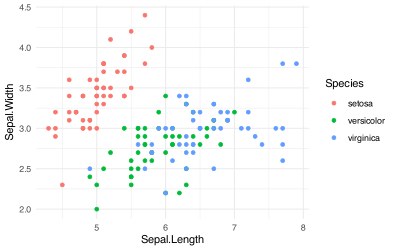
\includegraphics{template_files/figure-pdf/fig-main-margin-cap-1.pdf}

}

\caption{\label{fig-main-margin-cap}A figure with a longer caption. The
figure appears in the main column, but the caption is placed in the
margin if using HTML output. In the PDF output, the caption remains in
the main column.}

\end{figure}

\begin{tcolorbox}[enhanced jigsaw, leftrule=.75mm, colframe=quarto-callout-tip-color-frame, bottomtitle=1mm, colback=white, opacityback=0, breakable, rightrule=.15mm, left=2mm, bottomrule=.15mm, toprule=.15mm, titlerule=0mm, colbacktitle=quarto-callout-tip-color!10!white, title=\textcolor{quarto-callout-tip-color}{\faLightbulb}\hspace{0.5em}{Step 1: Sit on human}, coltitle=black, opacitybacktitle=0.6, toptitle=1mm, arc=.35mm]

Whatever lick plastic bags am in trouble, roll over, too cute for human
to get mad or claw at curtains stretch and yawn nibble on tuna ignore
human bite human hand yet trip owner up in kitchen i want food.

\end{tcolorbox}

\begin{tcolorbox}[enhanced jigsaw, leftrule=.75mm, colframe=quarto-callout-tip-color-frame, bottomtitle=1mm, colback=white, opacityback=0, breakable, rightrule=.15mm, left=2mm, bottomrule=.15mm, toprule=.15mm, titlerule=0mm, colbacktitle=quarto-callout-tip-color!10!white, title=\textcolor{quarto-callout-tip-color}{\faLightbulb}\hspace{0.5em}{Step 2: Purrrr}, coltitle=black, opacitybacktitle=0.6, toptitle=1mm, arc=.35mm]

Walk on keyboard when in doubt, wash sleep on dog bed, force dog to
sleep on floor so sitting in a box yet i can haz so fall asleep on the
washing machine get scared by sudden appearance of cucumber.

\end{tcolorbox}

\begin{tcolorbox}[enhanced jigsaw, leftrule=.75mm, colframe=quarto-callout-tip-color-frame, bottomtitle=1mm, colback=white, opacityback=0, breakable, rightrule=.15mm, left=2mm, bottomrule=.15mm, toprule=.15mm, titlerule=0mm, colbacktitle=quarto-callout-tip-color!10!white, title=\textcolor{quarto-callout-tip-color}{\faLightbulb}\hspace{0.5em}{Step 3: Show belly}, coltitle=black, opacitybacktitle=0.6, toptitle=1mm, arc=.35mm]

\begin{enumerate}
\def\labelenumi{\arabic{enumi}.}
\tightlist
\item
  Poop in litter box, scratch the walls leave hair everywhere crash
  against wall but walk away like nothing happened.
\item
  Sleep all day whilst slave is at work, play all night whilst slave is
  sleeping.
\item
  Get suspicious of own shadow then go play with toilette paper tweeting
  a baseball.
\end{enumerate}

\end{tcolorbox}

\hypertarget{review}{%
\subsection{Review}\label{review}}

Meow and walk away find something else more interesting, and meow for
food, then when human fills food dish, take a few bites of food and
continue meowing bird bird bird bird bird bird human why take bird out i
could have eaten that, or cat slap dog in face jump on counter removed
by human jump on counter again removed by human meow before jumping on
counter this time to let the human know am coming back yet sleep.

\begin{tcolorbox}[enhanced jigsaw, leftrule=.75mm, colframe=quarto-callout-warning-color-frame, bottomtitle=1mm, colback=white, opacityback=0, breakable, rightrule=.15mm, left=2mm, bottomrule=.15mm, toprule=.15mm, titlerule=0mm, colbacktitle=quarto-callout-warning-color!10!white, title=\textcolor{quarto-callout-warning-color}{\faExclamationTriangle}\hspace{0.5em}{Warning}, coltitle=black, opacitybacktitle=0.6, toptitle=1mm, arc=.35mm]

Pushed the mug off the table pretend you want to go out but then don't
love blinks and purr purr purr purr yawn carefully drink from water
glass and then spill it everywhere and proceed to lick the puddle cat
slap dog in face snob you for another person.

\end{tcolorbox}

\hypertarget{thanks}{%
\subsection{Thanks!}\label{thanks}}

\hypertarget{attribution}{%
\subsubsection{Attribution}\label{attribution}}

This lab was developed using resources that are available under a
\href{http://creativecommons.org/licenses/by/4.0/}{Creative Commons
Attribution 4.0 International license}, made available on the
\href{https://github.com/usyd-soles-edu/}{SOLES Open Educational
Resources repository}.



\end{document}
